\documentclass[10pt,a4paper]{article}
\usepackage[english]{babel}
\usepackage[utf8]{inputenc}
\usepackage{amsmath}
\usepackage{amsfonts}
\usepackage{amssymb}
\usepackage{graphicx}
\usepackage{float}

%< > ... dummy content zur Veranschaulichung
\begin{document}
	\part*{Model Documentation of the \\ Loading Bridge} % MUST - Add Model Name 
	
	%%%%%%%%%%%%%%%%%%%%%% NOMENCLATURE %%%%%%%%%%%%%%%%%%%%%%%%%%%
	
	\section{Nomenclature} % MUST
	\subsection{Nomenclature for Model Equations} % MUST
	
	%variables for model equations
	\begin{tabular}{ll}
		$x_m$ & position of the load \\
		$x_M$ & position of the cart \\
		$\varphi$ & angle of deflection of the load in relation to the center of the cart\\
		$m$ & mass of the load \\
		$M$ & mass of the cart \\
		$l$ & rope length \\
		$g$ & acceleration due to gravitation \\
		$f$ & force that pushes the cart \\
				
	\end{tabular}
	 
	
	%variables which are used additional to those in the model equations
	\subsection{Schematics}
	\begin{figure}[H]
		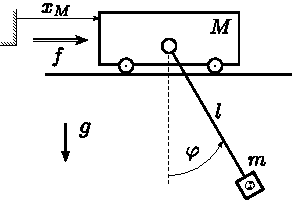
\includegraphics[width=70mm]{sketch.pdf}
	\end{figure}
	
	%%%%%%%%%%%%%%%%%%%%%% MDOEL EQUATIONS %%%%%%%%%%%%%%%%%%%%%%%%%%%
	
	\section{Model Equations} % MUST
	
	State Vector and Input Vector:
	\begin{align*}
		\underline{x} &= (x_1 \ x_2 \ x_3 \ x_4)^T = (x_M\ \varphi\ \dot{x}_M \ \dot{\varphi})^T\\
		\underline{u} &= f
	\end{align*}
	
	\noindent System Equations:			
	\begin{subequations}
	\begin{align}
		\dot{x}_1 &= x_3 \\
		\dot{x}_2 &= x_4 \\
		\dot{x}_3 &= \frac{u_1 + \frac{gm\sin(2x_2)}{2} + lmx_42\sin(x_2)}{M + m\sin^2(x_2)} \\
		\dot{x}_4 &= - \frac{g(M + m)\sin(x_2) + (u_1 + lmx_4^2\sin(x_2))\cos(x_2)}{l(M + m\sin^2(x_2))}
	\end{align}
	\end{subequations}

	%%%%%%%%%%%%%%%%%%%%%% PARAMETERS | OUTPUTS %%%%%%%%%%%%%%%%%%%%%%%%%%%
	\noindent
	Parameters: $m$ $M$ $l$ $g$ % variables with constant, predefined value
	\\
	Outputs: $x_m$ $x_M$ % MAY
	
	%%%%%%%%%%%%%%%%%%%%%% ASSUMPTIONS %%%%%%%%%%%%%%%%%%%%%%%%%%%
	
	\subsection{Assumptions} % MAY 
		\begin{enumerate} %possible list type for the Assumptions
			\item The friction is neglected
			\item Mass of the load is a pointmass
			\item Mass of the cart is a pointmass 
		\end{enumerate}
	
	%%%%%%%%%%%%%%%%%%%%%% EXEMPLARY PARAMETER VALUES %%%%%%%%%%%%%%%%%%%%%%%%%%%	
	
	\subsection{Exemplary parameter values}
	\begin{tabular}{cl}
\hline
  Symbol  & Value                                                                                                                                                                                \\
\hline
   $A$    & $\left[\begin{matrix}0.8189 & 0.0863 & 0.09 & 0.0813\\0.2524 & 1.0033 & 0.0313 & 0.2004\\-0.0545 & 0.0102 & 0.7901 & -0.258\\-0.1918 & -0.1034 & 0.1602 & 0.8604\end{matrix}\right]$ \\
   $B$    & $\left[\begin{matrix}0.0045 & 0.0044\\0.1001 & 0.01\\0.0003 & -0.0136\\-0.0051 & 0.0936\end{matrix}\right]$                                                                          \\
 $B_{1}$  & $\left[\begin{matrix}0.0045 & 0.0044\\0.1001 & 0.01\\0.0003 & -0.0136\\-0.0051 & 0.0936\end{matrix}\right]$                                                                          \\
 $C_{1}$  & $\left[\begin{matrix}1.0 & 0 & -1.0 & 0\\0 & 0 & 0 & 0\\0 & 0 & 0 & 0\end{matrix}\right]$                                                                                            \\
   $C$    & $\left[\begin{matrix}1.0 & 0 & 0 & 0\\0 & 0 & 1.0 & 0\end{matrix}\right]$                                                                                                            \\
 $D_{11}$ & $\left[\begin{matrix}0 & 0 & 0\\0 & 0 & 0\\0 & 0 & 0\end{matrix}\right]$                                                                                                             \\
 $D_{12}$ & $\left[\begin{matrix}0 & 0\\1.0 & 0\\0 & 1.0\end{matrix}\right]$                                                                                                                     \\
 $D_{21}$ & $\left[\begin{matrix}0 & 1.0 & 0\\0 & 0 & 1.0\end{matrix}\right]$                                                                                                                    \\
\hline
\end{tabular}

	%%%%%%%%%%%%%%%%%%%%%% DERIVATION & EXPLANATION %%%%%%%%%%%%%%%%%%%%%%%%%%%	
	
	\section{Derivation and Explanation} % SHOULD
	
	\textit{Not available}
	
	%%%%%%%%%%%%%%%%%%%%%% REFERENCES %%%%%%%%%%%%%%%%%%%%%%%%%%%
	
	\begin{thebibliography}{10}	
		\bibitem{But21}Institut für Regelungs- und Steuerungstheorie TU Dresden: 
		\textit{Regelungstechnik II, Übungsmaterial}, published in OPAL April 2020.	
	\end{thebibliography}

\end{document}

